\documentclass{beamer}
\usepackage[spanish]{babel}
\usepackage[utf8]{inputenc}
\usepackage{graphicx}

\title[La bisección de $f(x)=cos($\pi$x)$ en \textsc{Beamer}]{Bisección con $f(x)=cos($\pi$x)$}
\author[D. Montesdeoca y  L. Martín]{Carmen Laura Martín González
y
David Tomás Montesdeoca Flores}
\date[11/05/14]{11 de mayo de 2014}
\usetheme{Madrid}


\begin{document}

\begin{frame}
\titlepage
\end{frame}

\begin{frame}
\frametitle{Indice}
\tableofcontents[pausesections]

\end{frame}

\section{Definición de Bisección}

\begin{frame}
\frametitle{Definición de Bisección}

Según la RAE, La bisección es la acción o efecto de bisecar,es decir, dividir a la mitad y se aplica generalmente en la división de ángulos. Aunque esta definición no se aleja mucho de la deseada, la que verdaderamente nos interesa es la siguiente:

\begin{block}{Definición aplicada}
El método de bisección es un algoritmo usado en matemáticas para llevar a cabo una búsqueda de raíces. En resumen, este método encuentra una raíz de $f(x)=0$. Este método se realiza dividiendo el intervalo a la mitad y seleccionando el subintervalo de estos que contiene la raíz, que es aquel en el que hay un cambio de signo.(Se sabe que una raíz esta en un intervalo cerrado si la función cambia de signo en los puntos extremos). Cuantas más cifras decimales queramos obtener más divisiones tendremos que realizar.
\end{block} 

\end{frame}

\section{Definición del número $\pi$}

\begin{frame}
\frametitle{Definición del número $\pi$}
\begin{block}{Definición}
El número $\pi$ es la relación existente entre el diámetro de la circunferencia con su longitud.
Es un número irracional de los más importantes usados en las ciencias matemáticas, como la física, las ingenierías y las propias matemáticas.

El valor que toma esta constante es aproximadamente:
 $$\pi = 3.14159265358979323846...$$
\end{block}
El número $\pi$ se puede calcular mediante integración:

$$\int_{0}^{1} \! \frac{4}{1+x^2}\, dx = 4(atan(1) -atan(0)) = \pi $$

\end{frame}

\section{Ejemplo general de bisección}

\begin{frame}
\frametitle{Ejemplo general de bisección.}

\begin{block}{}
En la figura, se muestra gráficamente como los valores sucesivos convergen en una raíz de $f(x)$ cuando se empiezan con un par de valores que encierran una raíz. Podemos ver que 5.5 está a la mitad entre 4 y 6, y que 5.75 a la mitad entre 5.5 y 6. Siempre se considera al siguiente valor x al punto medio del último par que encierra entre corchetes a la raíz: Estos valores encierran a la raíz cuando $f(x)$ cambia de signo en los dos puntos.
\end{block}

\begin{figure}[b]
\begin{center}
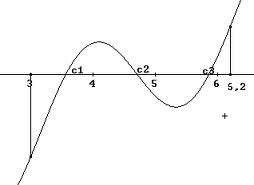
\includegraphics[scale=0.4]{images.jpeg}
\end{center}
\end{figure}

\end{frame}

\section{Teorema de bisección}

\begin{frame}
\frametitle{Teorema de Bisección}
\begin{block}{Teorema}
Si $[a_0, b_0],[a_1,b1],...,[a_n,b_n],...,$ denotan los intervalos en el método de la bisección, entonces los límites $\lim_{n\rightarrow \infty} a_n$ y $\lim_{n\rightarrow \infty}b_n $ existen , son iguales y representan un cero de f. Si r=$\lim_{n\rightarrow \infty}c_n$ y $c_n=(a_n+b_n)$ entonces: $$\|r-c_n\|<=2^{-(n+1)} (b_0 - a_0)$$
\end{block}

\end{frame}


\section{Algunas fórmulas que contienen el número $\pi$}
\subsection{Geometría} 

\begin{frame}
\frametitle{Algunas fórmulas que contienen el número $\pi$} 

\begin{block}{Geometría}

\begin{itemize}

  \item Longitud de la circunferencia.
  \pause
  \item Área del círculo.
  \pause
  \item Área interior de la elipse.
  \pause
  \item Área del cono.
  \pause
  \item Área de la esfera.

\end{itemize}
\end{block}

\end{frame}

\subsection{Análisis}
\begin{frame}
\frametitle{Algunas fórmulas que contienen el número $\pi$}
\begin{block}{Análisis}
\begin{itemize}
  \item Fórmula de Leibniz.
  \pause
  \item Producto de Wallis.
  \pause
  \item Fórmula de Euler.
  \pause
  \item Fórmula de Stirling.
  \pause
  \item Método de Montecarlo

\end{itemize}
\end{block}

\end{frame}

\subsection{Cálculo} 
\begin{frame}

\begin{block}{Cálculo}
\begin{itemize}
  \item Área limitada por la astroide: $\frac{3}{8}\pi a^2 $.
  \pause

  \item Área de la región comprendida por el eje X y un arco de la cicloide: $3 \pi a^2.$

\end{itemize}
\end{block}

\end{frame}

\begin{frame}
\frametitle{Bibliografía}
\begin{thebibliography}
  \beamertermplatebookbibitems
  \bibitem[Internet]{wikipedia}
  {\small $es.wikipedia.org/wiki/Método\_de\_bisección\#Algoritmo$}
  
  \beamertermplatebookbibitems
  \bibitem[Internet]{Juegos de lógica}
  {\small $www.juegosdelogica.com/numero\_\pi.htm$}
  
  \beamertermplatebookbibitems
  \bibitem[Internet]{Juegos de lógica}
  {\small $Análisis Numérico con Aplicaciones. Gerald·Wheatley. Editorial: Prentice Hall$}
  
\end{thebibliography}
\end{frame}

\end{document}
